
\Gls{ml} is the application of statistics, algorithms and computing power to discover meaning and/or devise actions from data.
\gls{ml} has become an umbrella term, encompassing the family of algorithms
    which aim to leverage computers to learn without being explicitly programmed,
    as opposed to the more general \gls{ai}, which seeks to make computers behave intelligently,
    admitting explicit programs to achieve tasks \cite{MLvAI}.
Its history is therefore imprecise since a number of early, apparently unrelated algorithms were proposed independently, 
    which now constitute \gls{ml} routines \cite{mcculloch1943logical, turing2009computing}. 
Nevertheless, the field of \gls{ml} has been advancing rapidly since the second half of the $20^{\textrm{th}}$ century \cite{russell2002artificial}, 
    especially recently due to the availability of advanced hardware such as \glspl{gpu}, 
    facilitating significant progress through an ever-increasing aresnal of powerful open source software \cite{pedregosa2011scikit, abadi2016tensorflow, paszke2019pytorch}. 
\par 

Throughout this thesis, we endeavour to combine known methods from the \gls{ml} literature with capabilities of \glspl{qc}\footnotemark. 
Typical \gls{ml} algorithms, which rely on \glspl{cpu} or \glspl{gpu}, are deemed \emph{classical} \acrlong{ml},
    in contrast with \gls{qml}, where \glspl{qc} are central to processing the data.
Similarly to the remit of \cref{chapter:qm}, here we do not provide an exhaustive account of \gls{ml} algorithms;
    we describe only the concepts which are used in later chapters, 
    referring readers to standard texts for a wider discussion \cite{russell2002artificial, hastie2009elements}.

\footnotetext{Or simulated \glspl{qc}, in this thesis.}


\section{Classical machine learning}\label{sec:classical_ml}

The first step in any \gls{ml} application is to consider the ensemble of known algorithms, 
    with respect to the available data.
Classical \gls{ml} is usually described in three categories:
    \emph{supervised learning}, \emph{unsupervised learning} and \emph{reinforcement learning}.  
These categories are broadly based on the format of data on which the insight can be built;
    we will briefly describe each to provide context to discussions throughout this thesis. 
Later in this thesis we will use the word \emph{model} for descriptions of quantum systems, 
    but here \emph{model} refers to the mapping between inputs and outputs, devised by the \gls{ml} algorithm.
\par 

\subsection{Supervised machine learning}
Models are trained using \emph{labelled} data, 
    i.e. each training sample has a known label $y_i$ -- 
    or, a set of \emph{feature vectors} $\left\{\vec{x}_i\right\}$ are associated with the set of 
    corresponding \emph{classes} $\left\{ y_i \right\}$ \cite{caruana2006empirical}. 
The output is a predictive tool which aims to reconstruct the classes of unseen feature vectors:
    in general, we can view the role of \gls{ml} in this setting as distilling the function $f$ such that 
\begin{equation}
    \label{eqn:supervised_ml_target}
    f : \vec{x}_i \longmapsto y_i \ \ \ \  \forall (\vec{x}_i, y_i).
\end{equation}
\par 

\par 

There are a number of families of algorithms even within the broad category of supervised \gls{ml},
    we define them as follows.
\begin{description}
    \item[Classification] \ 
    
        Algorithms that aim to produce models which can assign unseen instances to the most appropriate label,
        from a fixed set of available labels  \cite{kotsiantis2007supervised}.
        \begin{easylist}[itemize]
            && For example, labels indicate animals' species, and the feature vector for each sample (data point) 
            encodes the animals' height, weight, number of legs, etc. 
        \end{easylist}
    \item[Regression] \ 
    
        Models which capture the formulaic relationship -- either linear or polynamial -- 
            between numerical features and a target scalar value, 
            by determining coefficients for each feature. 
        \begin{easylist} 
            && For example, $y$ is the salary of employees in a company, and the feature vector consists of 
            the individual employees' age, seniority, experience in years, etc. 
        \end{easylist}

    \item[Neural networks] \ 
    
        \emph{Universal function approximators}\footnotemark.
        \footnotetext{Including {deep learning} networks \cite{hinton2006fast}.}
        By invoking a set of linear and non-linear transformations on input data, 
        the \emph{network} is a function of some paramterisation $w$;
        neural networks aim to find the optimal network, $w^{\prime}$, such that \cref{eqn:supervised_ml_target} is satisfied, 
        $f(w^{\prime}): \vec{x}_i \longmapsto y_i$. 
        \begin{easylist}
            && Usually used for classification.
            && For example, input \emph{neurons}\footnotemark \ encode the pixel values of images. 
            The neural network can be used to classify the objects it detects within the image. 
        \end{easylist}

    \item[ Support Vector Machines ] \ 
        
        Distinguish similar data points by projecting data into higher dimensional space,
        and therein finding the hypersurface which separates classes \cite{boser1992training}.
        \begin{easylist}
            && Usually used for classification tasks.
            && For data $\mathcal{D} \in \mathbb{R}^n$, a hypersurface in $\mathbb{R}^{n-1}$, 
                can be drawn arbitrarilily through the space (e.g. a 2D plane in a 3D space).
            && Unseen data can then classified by which partition they reside in when projected into the $n$-dimensional space.
            && The task of the support vector machine is to orient the hypersurface in such a way as to separate distinct classes.                 
        \end{easylist}
\end{description}

\footnotetext{
    The term \emph{neuron}, also known as \emph{node} or \emph{unit}, 
    derives from the motivation for this class of algorithm: the cells in the brain used for processing information. 
}
\par 

Supervised \gls{ml} algorithms rely on the existence of a body of labelled samples 
    -- the dataset $\mathcal{D}$ -- upon which the model can be trained.
Training is typically performed on a subset of the data, $\mathcal{D}_t$, usually 80\% of samples chosen at random. 
The remaining (20\%) of samples, $\mathcal{D}_v$, are retained for the evaluation of the resultant model: 
    $d \in \mathcal{D}_v$ are not trained upon, so do not contribute to the structure of $f$ as returned by the algorithm.
    The model therefore can not \emph{overfit}, i.e. simply recognise particular samples and label them correctly,
    without any meaningful inference. 
The evalutation thus captures how the model can be expected to perform on future, unlabelled data. 
\par 

\subsubsection{Performance metrics}\label{sec:performance_metrics}
The fair assessment of supervised methods can be achieved through a number of \emph{performance metrics}.
In each supervised \gls{ml} algorithm, the machine attempts to learn the structure of $f$ that optimises some internal \gls{of}, 
    e.g. minimising the average distance between predicted and target labels for regression, $\sum\limits_{d \in \mathcal{D}_t} y_d - y^{\prime}_d$.
To assess the resultant model, we introduce a number of \emph{performance metrics}, 
    which aim to measure serveral perspectives of the model's efficacy, by considering the model's predictions with respect to $\mathcal{D}_v$. 
\par 

By definition of the data format, it is relatively straightforward to define metrics for supervised routines:
    the classes assigned to feature vectors, $y_i^{\prime}$, can be quantitatively assessed with respect to their true class, $y_i$. 
For example, in \emph{binary classification}, the output of the model is either correct or incorrect, 
    allowing us to meaningfully assess its average performance. 
Likewise, for numerical targets, the difference $\absval{y_i - y_i^{\prime}}$ 
    for each sample cumulatively indicate the strength of the model. 
\par 



There are a large number of quantities and performance metrics against which to judge models' outputs.
In binary classification, we care about whether the model predicts that a given feature is present,
    and whether it predicts features incorrectly. 
For example, the model aims to classify whether or not a dog is present in an image. 
These type of binary predictions have four outcomes, which can be summarised in a \emph{confusion matrix} (\cref{fig:confusion_matrix}), 
    defined as in \cref{table:classification_metrics}.
\begin{figure}[t]
    \begin{center}
        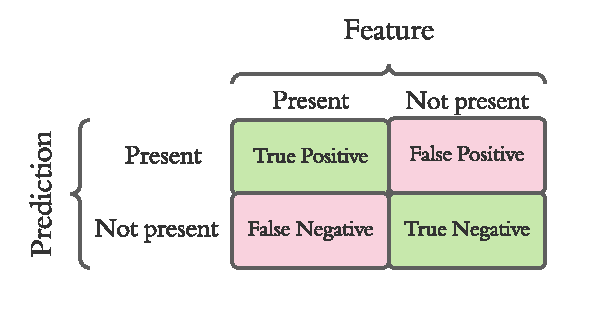
\includegraphics{contextual_review/figures/confusion_matrix.pdf}
    \end{center}
    \caption[Confusion matrix]{
        Confusion matrix showing the meaning of 
        \acrlong{tp}, \acrlong{tn}, \acrlong{fp} and \acrlong{fn}.
    }
    \label{fig:confusion_matrix}
\end{figure}
    
\begin{table}[H]
    \begin{center}
    \begin{tabular}{lcc}
        & $y$ has feature & $y^{\prime}$ has feature \\
        \hline
        \Acrfull{tp} & \tick & \tick \\
        \Acrfull{fp} & \cross & \tick \\
        \Acrfull{tn} & \cross & \cross \\
        \Acrfull{fn} & \tick & \cross\\
    \end{tabular}
    \end{center}
    \caption[Classification metrics]{
        Classification metrics. 
        We define classification outcomes based on whether the considered feature was present and/or predicted. 
    }
    \label{table:classification_metrics}
\end{table}
\par 
    
We can use the concepts of \cref{table:classification_metrics} to define a series of \emph{rates} 
    which characterise the model's predictions. 
    
\begin{description}\label{description:ml_metrics}
    \begin{subequations}
    \item[Accuracy] The overall rate at which the algorithm predicts the correct result. 
    \begin{equation}\label{eqn:accuracy_eqn}
        \textrm{accuracy} = \frac{\tp + \tn}{\tp + \tn + \fn + \fp}
    \end{equation}
    
    \item[Precision] Positive predicitve rate. Of those \emph{predicted to have} the feature of interest, what percentage \emph{actually have} the feature. 
    \begin{equation}\label{eqn:precision_eqn}
        \textrm{precision} = \frac{\tp}{\tp+\fp}
    \end{equation}
    
    \item[Sensitivity] True positive rate (also known as \emph{recall}). Of those which \emph{actually have} the feature, what percentage are \emph{predicted to have} the feature.
    \begin{equation}\label{eqn:sensitivity_eqn}
        \textrm{sensitivity} = \frac{\tp}{\tp+\fn}
    \end{equation}
    
    \item[Specificity] True negative rate. Of those which  \emph{do not actually have} the feature of interest, how many are \emph{predicted not to} have the feature.
    \begin{equation}\label{eqn:specificity_eqn}
        \textrm{specificity} = \frac{\tn}{\tn+\fp}
    \end{equation}
    \end{subequations}
\end{description}
    
Each metric has clear advantages, but consider also their drawbacks:
\begin{easylist}[itemize]
    & Accuracy can be extremely misleading. 
        For example, consider a dataset of 10,000 samples, of which only 100 contain the feature of interest.
        A binary model which predicts every instance as \ttt{False} will achieve $\tn=9,900, \fn=100$, 
            receiving an overall $\textrm{accuracy}=99\%$, despite not having found a single positive sample. 
        This is clearly not useful in identifying the minority of cases of actual interest. 
    & Sensitivity can be inflated by over-fitting to positive cases. 
        That is, by predicting the feature as present in all cases, all true instances of the feature will be found, 
        however all \ttt{False} instances will be labelled as having the feature, 
        so the model has not helped separate the data.
        The model willl yield a high rate of \gls{tp} but also a high rate of \gls{fp}. 
    & Precision can be high for extremely selective models, i.e. those which are conservative in predicting the presence of the feature.
        By predicting relatively few positive instances, it can ensure that a high proportion of its predictions are correct. 
        The absolute number of instances identified, however, is relatively low as a proportion of the total number in the dataset. 
    & Specificity, similar to sensitivity, can easily mislead by identifying very few instances as having the target feature. 
        Then, it will correctly predict most non-present instances as \ttt{False}, but will not identify the few instances of interest.  
\end{easylist}

Clearly, the performance metric must be chosen with due consideration for the application;
    e.g. in testing for a medical condition, rather than incorrectly telling a patient they do not have the condition because the 
    model predicted they were feature-negative, it is preferable to incorrectly identify some patients as feature-positive (since they can be retested). 
In this case, high accuracy is crucial, at the expense of precision. 
It is appropriate to blend together these metrics, in order to derive performance metrics which balance the priorities of the outcomes.
In general -- including in this thesis -- the most important aspects of a \gls{ml} are precision and sensitivity: 
    a model which performs well with respect to \emph{both} of these is sensitive to the feature, but precise in its predictions. 
A quantity which captures both of these is the $F_{\beta}$-score, 
\begin{equation}\label{eqn:f_beta}
    f_{\beta} = \left( 1 + \beta^2 \right) \frac{
        \textrm{precision} \times \textrm{sensitivity} }{
        \left(\beta^2\times\textrm{precision}\right) + \textrm{sensitivity}},
\end{equation}
where $\beta \in \mathbb{R}$ is the relative weight of priority of sensitivity with respect to precision. 
In particular, considering precision and sensitivity as equally important, i.e. $\beta=1$, 
    we have the \gls{fscore}, 
\begin{equation}
    \label{eqn:f_score_def}
    f_1 = \frac{2 \times \textrm{precision} \times \textrm{sensitivity} }{\textrm{precision} + \textrm{sensitivity}}.
\end{equation}
For examples of how \gls{fscore} balances these considerations, see \cref{table:f1_example}.
\par

\begin{table}[t]
    \centering
    \begin{tabular}{|ccc|cc|c|}
        \hline
        \Acrlong{tp} & \Acrlong{fn} & \Acrlong{fp} & Precision & Sensitivity & \gls{fscore}  \\
        \hline
        \rule{0pt}{3ex} 500 & 500 & 1000 & 33 & 50 & $ (\frac{2 \times 33 \times 50 }{33 + 50 }) = 37 $ \\
        \rule{0pt}{3ex} 500 & 500 & 500 & 50 & 50 & $( \frac{2 \times 50 \times 50 }{50 + 50 } ) = 50 $ \\
        \rule{0pt}{3ex} 1000 & 0 & 1000 & 50 & 100 & $ (\frac{2 \times 50 \times 100} { 50 + 100 }) = 67 $ \\
        \rule{0pt}{3ex} 1000  & 0 & 0 & 100 & 100 & $ (\frac{2 \times 100 \times 100}{100 + 100}) = 100 $ \\
        \hline
    \end{tabular}
    \caption[$F_1$-score examples]{
        Examples of how \gls{fscore} behaves for varying \acrlong{tp}, \acrlong{fn} and \acrlong{fp}. 
    }
    \label{table:f1_example}
\end{table}


\subsection{Unsupervised machine learning}

Contrary to supervised algorithms, unsupervised methods operate on \emph{unlabelled} data, $\mathcal{D}$. 
This is often summarised as finding structure within unstructured data.
Although we do not utilise these methods in this thesis, we briefly summarise them here for completeness;
    again, we can further compartmentalise methods under this umbrella as follows \cite{geron2019hands}. 

\begin{description}
    \item[Clustering] \ 
    
    Finding datapoints which are similar to each other, according to some distance metric.
    \begin{easylist}
        && For example, online retailers grouping together customers with similar preferences, in order to tailor advertising campaigns. 
    \end{easylist}
    \item[Dimensionality reduction] \ 
    
    Reducing the feature vector of each sample in a dataset to its essential components,
        which may be amalgamations of original features, while retaining structure within the data.
    \begin{easylist}
        && This can be used for visualisation to allow for inspection of complex datasets, 
        e.g. plotting users of a social network as nodes on a 2D map, where distinct social groups
        are kept distant. 
    \end{easylist}
    \item[Association learning] \ 
    
    Discover correlations among data. 
    \begin{easylist}
        && For instance, a supermarket may find that purchasers of certain products are likely also to buy others, 
            providing actionable insight.
            For example, purchases involving bread also include butter in $50\%$ of cases, 
            so positioning these nearby may increase sales by reminding consumers of their compatibility. 
    \end{easylist}
    \item[Semi-supervised learning] \ 
    
    Combine elements of supervised and unsupervised algorithms, 
        to achieve a task beyond the remit of either alone. 
        This often means classifying data where only occur a small subset of the total dataset is labelled. 
    \begin{easylist}
        && e.g. in facial recognition, a clustering algorithm finds similarities between individual people in photos, 
            and identifies a single person present across a number of photos, and associates those photos together. 
            It combines this with a small set of photos for which people have been tagged, 
                locates the same person and automatically tags them in the wider set of photos. 
    \end{easylist}
\end{description}
\par 

\subsection{Reinforcement learning}
A third category of \gls{ml} algorithms are reinforcement learning.
These are methods where an \emph{agent} interacts with some environment, 
    and refines a \emph{policy} for reacting to different stimuli. 
As such, the agent can, in principle, deal with a wide array of situations. 
These methods underly technologies such as self-driving cars, 
    which inspect their surroundings through \emph{sensors};
    compute an \emph{action} according to the policy, 
    and implement that action through \emph{actuators}.
Following an action, the agent senses whether that action was beneficial or detrimental, 
    and receives a \emph{reward} or \emph{punishment} accordingly. 
Highly rewarded actions are likely to be repeated in future, allowing the agent to learn what response is 
    appropriate to situational parameters, 
    e.g. a self-driving car braking at a red light is rewarded, 
    while braking at a green light is punished. 
\par 
The concept of a machine's \emph{agency} is an ongoing discussion in the \gls{ml} community \cite{franklin1996agent, wooldridge2009introduction}, 
    and will be important in this thesis when we define our model learning protocol as an agent;
    we will revisit the concept in \cref{sec:agency}.

\section{Quantum machine learning}\label{sec:quantum_machine_learning}
A growing domain is the development of \gls{ml} algorithms which run on quantum hardware, 
    or exploit data from quantum systems; generally referred to as \acrfull{qml} \cite{biamonte2017quantum, adcock2015advances}. 
There are a number of methodologies which are referred to as \gls{qml};
    for clarity, we define the main branches here, as shown in \cref{fig:qml_types}. 

\begin{description}\label{description:qml}
    \item[Classical machine learning] \ 

        Standard \gls{ml} as described in \cref{sec:classical_ml}, i.e. where the processors are \glspl{cpu} or \glspl{gpu}, 
            and the applications are not of specific interest to problems in the quantum domain. 
        Recently, this branch has encompassed quantum \emph{inspired} \gls{ml}, which still target classical problems, 
            but use subroutines which were orginally found in the context of \gls{qml} \cite{tang2019quantum}.

    \item[Quantum enhanced machine learning] \
    
        A quantum co-processor is leveraged on classical data for some provable speedup,
        i.e. data that could otherwise be processed purely classically, is encoded, loaded onto and processed by quantum hardware.
        The quantum counterparts of classical \gls{ml} algorithms aim to solve the same problems, 
            e.g. as neural networks \cite{schuld2014quest, cao2017quantum} and principal component analysis \cite{lloyd2014quantum}. 

    \item[Classical learning for quantum systems] \ 
    
        Classical processors are employed to extract insight on problems arising from quantum systems, 
            e.g. data is taken from a quantum system and analysed via purely classical methods.
            For instance, methods which aim to represent quantum states efficiently by leveraging 
            neural networks \cite{carleo2017solving, torlai2018neural}. 

    \item[Complete quantum machine learning] \ 

        Data of a quantum nature is processed -- at least partially -- by quantum processors. 
        The most common technique here is \gls{vqe}, which simulates quantum systems on \glspl{qc}, 
        in order to retrieve quantum systems' ground states \cite{peruzzo2014variational}.
        The algorithm relies on a classical optimisation routine, but was devised explicitly for implementation on quantum hardware. 
\end{description}
\begin{figure}[t]
    \begin{center}
        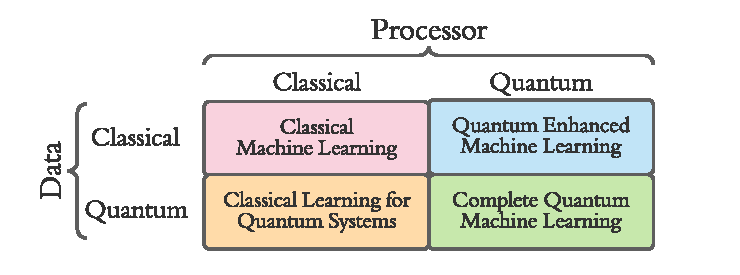
\includegraphics{contextual_review/figures/qml_types.pdf}
    \end{center}
    \caption[Types of quantum machine learning]{Types of \acrlong{qml}.}
    \label{fig:qml_types}
\end{figure}

\par 

The algorithms described in \cref{part:algorithms} and the applications in \crefrange{part:theoretical_study}{part:experimental_study}
    can be described as classical learning for quantum systems. 
This is because the data upon which the applications are built represent quantum systems, 
    but are processed through classical \gls{ml} algorithms in order to derive insight about those systems.
We caveat that it is feasible, and indeed the long term intention of such algorithms, 
    to run in conjunction with a quantum co-processor, which would represent and evolve quantum systems, 
    but all processing presented here are through strictly classical architecture.

\section{Genetic algorithms}\label{sec:genetic_algorithms}
In later chapters (\cref{chapter:ga} and \cref{chapter:many_qubits}) 
    we will use a class of optimisation techniques known as
    \emph{evolutionary algorithms} \cite{back1996evolutionary, de2020evolutionary}.
In particular, \emph{\acrfullpl{ga}} are central to our primary applications.
Here we describe \glspl{ga} in general terms for reference throughout. 
\par 
\glspl{ga} work by assuming a given problem can be optimised, if not solved, by a single candidate 
    among a fixed, closed space of candidates, called the population, $\population$. 
A number of candidates are sampled at random from $\population$ into a single \emph{generation}, 
    and evaluated through some \acrfull{of}, which assesses the fitness of the candidates at solving the problem of interest. 
Candidates from the generation are then mixed together to produce the next generation's candidates: 
    this \emph{crossover} process aims to combine only relatively strong candidates, such that the average 
    candidates' fitness improve at each successive generation, 
    mimicing the biological mechanism whereby the genetic makeup of \emph{offspring} is an even mixture of both parents
    through the philosophy of \emph{survival of the fittest}. 
The selection of strong candidates as parents for future generations is therefore imperative; 
    in general parents are chosen according to their fitness as determined by the \gls{of}. 
Buidling on this biological motivation, much of the power of \glspl{ga} comes from the concept of \emph{mutation}: 
    while offspring retain most of the genetic expressions of their parents, some elements are mutated at random.
Mutation is crucial in avoiding local optima of the \gls{of} landscape
    by maintaining diversity in the examined subspace of the population.
\par 

\glspl{ga} are not defined either as supervised or unspervised methods;
    this designation depends on the \gls{of}. 
If candidates are evaluated with respect to labelled data, we can consider that \gls{ga} supervised, 
    otherwise unsupervised. 
Pseudocode for a generic \gls{ga} is given in \cref{alg:ga},
    but we can informally define the procedure as follows. 
Given access to the population, $\population$, 

\begin{easylist}[enumerate]\label{mark:informal_ga}
    \ListProperties(Numbers2=l, Numbers3=r)
    & Sample $N_m$ candidates from $\population$ at random
    && call this group of candidates the first generation, $\mu$. 
    & \label{ga:loop} Evaluate each candidate $\gamma_j \in \mu$
    && each $\gamma_j$ is assigned a fitness, $g_j$;
    && the fitness is computed through an \gls{of}, $g$ acting on the candidate, i.e. $g_j = g(\gamma_j)$. 
    & Map the fitnesses of each candidate, $\{g_j\}$, to selection probabilities for each candidate, $\{s_j\}$
    && e.g. by normalising the fitnesses, or by removing some poorly-performing candidates and then normalising. 
    & Generate the next generation of candidates
    && Reset $\mu = \{ \}$;
    && \label{ga:select} Select pairs of parents, $\left\{\gamma_{p_1}, \gamma_{p_2}\right\}$, from $\mu$
    &&& Each candidate's probability of being chosen is given by their $s_j$.
    && Cross over $\left\{\gamma_{p_1}, \gamma_{p_2}\right\}$ to produce children candidates, $\left\{\gamma_{c_1}, \gamma_{c_2}\right\}$
    &&& mutate $\gamma_{c_1}, \gamma_{c_2}$ according to some random probabilistic process;
    &&& keep $\gamma_{c_i}$ only if it is not already in $\mu$, to ensure $N_m$ unique candidates are tested at each generation.
    && until $|\mu| = N_m$, iterate to step (\ref{ga:select}.
    & Until the $N_g^{th}$ generation is reached, iterate to step \ref{ga:loop};
    & The strongest candidate on the final generation is deemed the solution to the posed problem. 
\end{easylist}


\begin{algorithm}
    \caption{Genetic algorithm}
    \label{alg:ga}
    \DontPrintSemicolon
    \KwIn{ $\population$ \tcp*[1]{Population of candidate solutions to given problem}}
    \KwIn{ $g()$ \tcp*[1]{function to compute objective funtion}}
    \KwIn{ $\ttt{map\_g\_to\_s}()$ \tcp*[1]{function to map fitness to selection probability}}
    \KwIn{ $\ttt{select\_parents}()$ \tcp*[1]{function to select parents among generation}}
    \KwIn{ $\ttt{crossover}()$ \tcp*[1]{function to cross over two parents to produce offspring}}
    \KwIn{ $\ttt{mutate}()$ \tcp*[1]{function to mutate offspring probabilistically}}
    \KwIn{ $N_g$ \tcp*[1]{number of generations}}
    \KwIn{ $N_m$ \tcp*[1]{number of candidates per generation}}\;

    \KwOut{$\gamma^{\prime}$ \tcp*[1]{strongest candidate}}\;
    
    $\mu \gets \ttt{sample} \left( \population, N_m\right)$\; 

    \For{$i \in 1, ..., N_g$}{
        \For{$\gamma_j \in \mu$ }{
            $g_j \gets g(\gamma_j) $ \tcp*[1]{assess fitness of candidate}
        }

        $\{ s_j \}  \gets \ttt{ map\_g\_to\_s}(\{g_j \})$ \tcp*[1]{map fitnesses to normalised selection probability}
        $\mu_c = \argmax\limits_{s_j} \{ \gamma_j \}$ \tcp*[1]{record champion of this generation}\;

        $\mu \gets \{ \}$ \tcp*[1]{empty set for next generation}

        \While{$| \mu | < N_m$}{
            $p_1, p_2 \gets \ttt{select\_parents}(\{s_j\})$ \tcp*[1]{choose parents based on candidates' $s_j$}
            $c_1, c_2 \gets \ttt{crossover}(p_1,p_2)$ \tcp*[1]{generate offspring candidates based on parents}
            $c_1, c_2 \gets \ttt{mutate}(c_1,c_2)$ \tcp*[1]{probabilistically mutate offspring}

            \For{$c \in \{c_1, c_2\}$ }{
                \If{$c \notin \mu$}{
                    $\mu \gets \mu \cup \{ c\}$ \tcp*[1]{keep if child is new} 
                }
            }
        }
    }

    $\gamma^{\prime} \gets \argmax\limits_{s_j}\{ \gamma_j \in \mu \}$ \tcp*[1]{strongest candidate on final generation}\;

    return $\gamma^{\prime}$

\end{algorithm}


\par 

Candidates are manifested as \emph{\glspl{chromosome}}, i.e. strings of fixed length, 
    whose entries, called  \emph{\glspl{gene}}, each represent some proposed element of the system.
In general, \glspl{gene} can have continuous values, although usually, and for all purposes in this thesis, 
    genes are binary, capturing simply whether or not the \gls{gene}'s corresponding feature is present 
    in the \gls{chromosome}. 

\begin{figure}[t]
    \begin{center}
        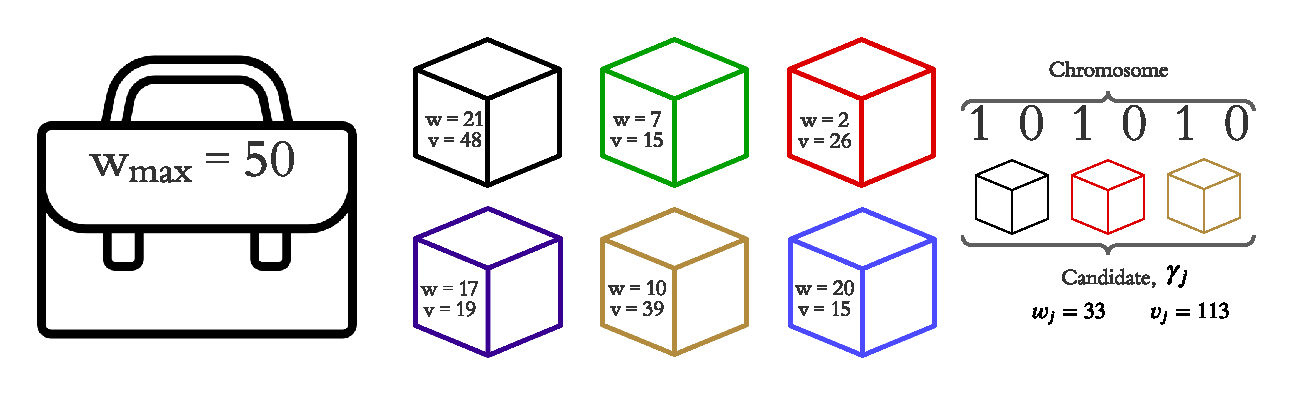
\includegraphics[width=\textwidth]{theoretical_study/figures/knapsack_schematic.pdf}
    \end{center}
    \caption[Knapsack problem]{
        Depiction of the knapsack problem.
        \textbf{Left}, A knapsack which can hold any number of objects but is constrained by the total weight it can support, 
        $w_{max} = 50$. 
        \textbf{Centre}, A set of objects are available, each with associated weight, $w$, and value $v$. 
        The objective is to find the subset of objects which maximise the total value, 
        while not exceeding the capacity of the knapsack. 
        \textbf{Right}, An example chromosome, i.e. candidate $\gamma_j$, where the bits of the chromosome indicate 
            whether the corresponding object is included, allowing for calculation of the total weight $w_j$ and value $v_j$ of 
            the candidate solution. 
    }

\end{figure}
\subsection{Illustrative example: knapsack problem}\label{sec:knapsack}
One commonly referenced combinatorial optimisation problem is the \emph{knacksack problem},
    which we will use to elucidate the abstract concepts described so far, 
    and introduce further concepts with immediate illustration. 
The knapsack problem is stated as:
    given a set of objects, where each object has a defined weight and value, 
    determine the set of objects to pack in a knapsack which can support a limited weight, 
    such that the value of the packed objects is maximised. 
Say there are $n$ objects;
    we can write the vector containing the values of those objects as $\vec{v}$, 
    and the vector of their weights as $\vec{w}$. 
We can then represent configurations of objects -- i.e. candidate solutions to the problem -- 
    as vectors $\vec{\gamma}_j$, whose elements are binary, 
    and simply indicate whether or not the associated object is included in the set. 
The candidate vector $\vec{\gamma}_j$ is equivalent to the chromosome $\gamma_j$. 
For example, with $n=6$,
\begin{equation}
    \vec{\gamma}_j = \irow{1 & 0 & 0 & 0 & 0 & 1} \Longrightarrow  \gamma_j = \ttt{100001} 
\end{equation} 
indicates a set of objects consisting only of those indexed first and last, with none of the intermediate objects included. 


\par
The fitness of any candidate is then given by the total value of that configuration of objects, $v_j = \vec{v} \cdot \vec{\gamma}_j$, 
    but candidates are only admitted if the weight of the corresponding set of objects 
    is less than the capacity of the knapsack\footnotemark \, i.e. $w_j = \vec{w} \cdot \vec{\gamma}_j \leq w_{max}$. 
\footnotetext{
    Note there are alternative strategies to dealing with candidates who violate the weight condition, 
    such as to impose a penalty within the \gls{of}, but for our purposes let us assume we simply disregard violators. 
}
\par 

For example where each individual object has value $<50$ and weight $<25$ and $w_{max} = 50$, 
recalling $\gamma_j = \ttt{100001}$, say, 
\begin{subequations}
    \begin{equation}
        \vec{ v } = \irow{ 48 & 15 & 26 & 19 & 39 & 15 } \Longrightarrow v_j = \vec{\gamma}_j \cdot \vec{v} = 48 + 15 = 63;
    \end{equation}
    \begin{equation}
        \vec{ w } = \irow{ 21 & 7 & 2 & 17 & 10 & 20 } \Longrightarrow w_j = \vec{\gamma}_j \cdot \vec{w} = 21 + 20 = 41.
    \end{equation}
\end{subequations}
We can hence assess the fitness of $\gamma_j$ as $63$ and deem it a valid candidate since it does not exceed the weight threshold.
We can likewise compute the total weight and value of a series of randomly generated candidates, 
    and deem them valid or not. 
\cref{table:knapsack_candidates} shows a set of 12 randomly generated candidates, 
    of which ten are valid.

\begin{table}
    \begin{center}
        \begin{tabular}{llrrl}
\hline
              &        &                                    Value &                                   Weight &                                    Valid \\
Name & Candidate &                                          &                                          &                                          \\
\midrule
$\gamma_{1}$ & 110011 &                                      117 &                                       58 &                                       No \\
$\gamma_{2}$ & 101010 &                                      113 &                                       33 &                                      Yes \\
$\gamma_{3}$ & 011110 &                                       99 &                                       36 &                                      Yes \\
$\gamma_{4}$ & 011011 &                                       95 &                                       39 &                                      Yes \\
$\gamma_{5}$ & 111000 &                                       89 &                                       30 &                                      Yes \\
$\gamma_{6}$ & 010111 &                                       88 &                                       54 &                                       No \\
$\gamma_{7}$ & 100010 &                                       87 &                                       31 &                                      Yes \\
$\gamma_{8}$ & 110001 &                                       78 &                                       48 &                                      Yes \\
$\gamma_{9}$ & 011101 &                                       75 &                                       46 &                                      Yes \\
$\gamma_{10}$ & 110000 &                                       63 &                                       28 &                                      Yes \\
$\gamma_{11}$ & 000011 &                                       54 &                                       30 &                                      Yes \\
$\gamma_{12}$ & 000101 &                                       34 &                                       37 &                                      Yes \\
\hline
\end{tabular}

        \caption[Candidate solutions to knapsack problem]{
            Candidate solutions to the knapsack problem for randomly generated chromosomes. 
        }
        \label{table:knapsack_candidates}
    \end{center}
\end{table}

The strongest (valid) candidates from \cref{table:knapsack_candidates} are \ttt{101010}, \ttt{011110}. 
We can combine these two strong candidates in order to produce further candidates:
    by merging the first half of the first candidate with the second half of the second candidate\footnotemark,
    we get the \emph{child} candidate $\gamma_{c} = \ttt{101110}$, 
    from which we can see $v_{c_1} = 132, w_{c_1} = 50$, 
    i.e. by combining two strong candidates we produce the strongest-yet-seen valid candidate. 
\footnotetext{This process is described as a one-point crossover in \cref{sec:reproduction} with this example shown in \cref{fig:gen_alg_reproduction}.}
\par 

By repeating this procedure, it is expected to uncover candidates which optimise $v_j$ while maintining $w_j \leq w_{max}$, 
    or at least to produce near-optimal solutions, using far less time/resources than brute-force evaluation of all candidates, 
    which is usually sufficient. 
For instance, with $n=100$ objects, there are $2^{100} \approx 10^{30}$ candidates to consider; 
    the most powerful supercomputers in the world currently claim on the order of Exa-FLOPs, 
    i.e. $10^{18}$ operations per second, of which say $\mathcal{O}(1000)$ operations are required to test each candidate, 
    meaning $10^{15}$ candidates can be checked per second in a generous example. 
This would still require $10^{12}$ seconds to solve absolutely, 
    so it is reasonable in cases like this to accept 
    \emph{approximately optimal} solutions\footnote{
        Simply put: in machine learning, \emph{good enough} is good enough.
        We will adopt this philosophy for the remainder of this thesis and life. 
    }. 


\subsection{Selection mechanism}

A key subroutine of every \gls{ga} is the mechanism through which it nominates candidates from generation $\mu$ 
as parents to offsping candidates in $\mu+1$ \cite{luke11}. 
All mechanisms have in common that they act on a set of candidates from the previous generation, 
    where each candidate, $\gamma_j$, has been evaluated and has fitness value, $g_j$. 
Among the viable schemes for selecting individual parents from $\mu$  are
\begin{easylist}[itemize]
    & Rank selection: candidates are selected with probabilty proportional to their ranking relative to 
        the fitness of contemporary candidates in the same generation;
    & Tournament selection: a subset of $k$ candidates are chosen at random from $\mu$, 
        of which the candidate with the highest fitness is taken as the parent;
    & Stochastic universal sampling: candidates are sampled proportional to their fitness, 
        but the sampling algorithm is biased to ensure high-fitness candidates are chosen at least once 
        within the generation. 
\end{easylist}

We will only detail the mechanism used in later applications within this thesis: 
    fitness proportional selection, known as \emph{roulette selection} \cite{luke11}. 
This is a straightforward strategy where we directly map candidates' fitness, $g_j$ to a selection probability, $s_j$,
    simply by normalising $\{g_i\}$, 
    allowing us to visualise a roulette wheel of uneven wedges, each of which correspond to a candidate. 
Then we need only conceptually spin the roulette wheel to select the first parent, $\gamma_{p_1}$. 
We then remove $\gamma_{p_1}$ from the set of potential parents, renormalise the remaining $\{s_j\}$, 
    and spin the wheel again to choose the second parent, $\gamma_{p_2}$. 
The roulette selection is shown in \cref{fig:knapsack_roulette}.
\par 

In practice, we repeat the roulette selection process outlined until the next generation is filled, 
    usually we have $|\mu| = N_m$, and desire that every generation should contain
    $N_m$ candidates, so we repeat the roulette selection $\nicefrac{N_m}{2}$ times per generation, 
    since every pair of parents yields two offspring.
It is important that meaningful differences in fitness are reflected by the selection probability, 
    which is difficult to ensure for large $N_m$, e.g. with 20 candidates, the strongest candidate is only 
    a marginally more probable parent than the worst -- this effect is amplified for larger $N_m$. 
We therefore wish to reduce the set of potential parents to ensure high quality offspring:
    we truncate $\mu$ with rate $\tau$ to retain only the $\tau N_m$ highest-fitness candidates as selectable parents.
\par 

\begin{figure}[t]
    \begin{center}
        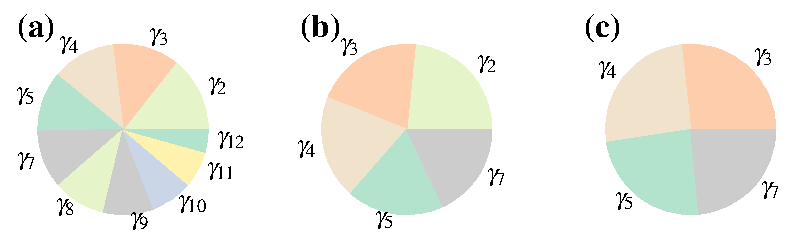
\includegraphics{theoretical_study/figures/knapsack_roulette.pdf}
    \end{center}
    \caption[Roulette wheels for selection]{
        Roulette wheels showing selection probability $s_j$ for corresponding candidates $\gamma_j$. 
        Colours here only distinguish candidates, they do not encode any information. 
        \textbf{a}, All valid candidates are assigned selection probability based on their value in \cref{table:knapsack_candidates}. 
        \textbf{b}, The set of potential parents is truncated to include only the strongest five candidates. 
        \textbf{c}, After one parent ($\gamma_2$) has been chosen, it is removed from the roulette wheel and the remaining
         candidates' probabilities are renormalised for the selection of the second parent. 
    }
    \label{fig:knapsack_roulette}
\end{figure}


\subsection{Reproduction}
\label{sec:reproduction}
\begin{figure}
    \begin{center}
        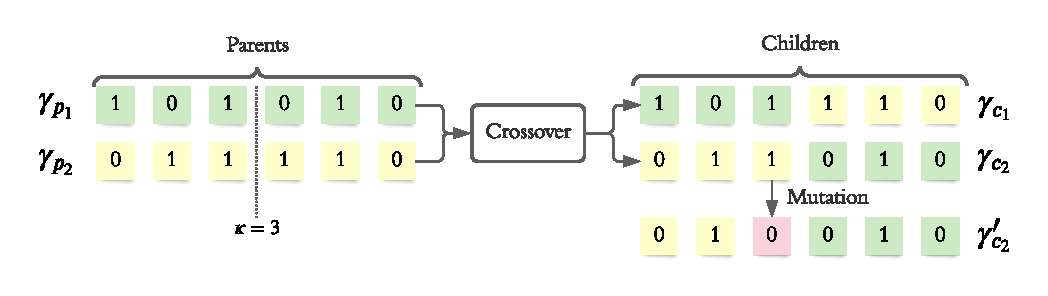
\includegraphics{theoretical_study/figures/chromosomes.pdf}
    \end{center}
    \caption[Crossover and mutation of chromosomes]{
        Crossover and mutation of chromosomes.
        Two parents, $\left\{\gamma_{p_1}, \gamma_{p_2}\right\}$, are nominated from the process in \cref{fig:knapsack_roulette}. 
        They are then crossed-over via a one-point crossover with crossing point $\kappa=3$, 
        resulting in children candidates $\left\{\gamma_{c_1}, \gamma_{c_2}\right\}$. 
        One child chromosome is mutated to yield a new candidate, $\gamma_{c_2}^{\prime}$. 
        The candidates added to the next generation are then $\{ \gamma_{c_1}, \gamma_{c_2}^{\prime} \}$.
    }
    \label{fig:gen_alg_reproduction}
\end{figure}

When a pair of parents have been nominated by the selection mechanism above, 
    it remains to use those parents to \emph{reproduce}, 
    i.e. to produce offspring which should inherit and improve upon the properties of their parents. 
Here we use a \emph{one-point crossover}, whereby the two parent chromosomes are mixed together 
    to form two offspring, about a single point, $\kappa$.
For candidates of $n$ genes, $\gamma_{c_1}$ is produced when
    the first $\kappa$ genes of $\gamma_{p_1}$ are conjoined with the latter $n - \kappa$ genes of $\gamma_{p_2}$;
    likewise $\gamma_{c_2}$ consists of the first $n-\kappa$ genes of $\gamma_{p_2}$ conjoined with the latter $\kappa$ genes of $\gamma_{p_1}$.
Often $\kappa$ is restricted to the midpoint of the chromosomes, although in general it need not be: 
    we will instead consider $\kappa \in \left( \frac{n}{4}, \frac{3n}{4} \right)$, 
    e.g. with $n=12$, $\kappa \in (3, 9)$. 
The one-point crossover is shown for $n=6$ with $\kappa=3$ in \cref{fig:gen_alg_reproduction}, 
    recalling the chromosome structure from \cref{fig:gen_alg_reproduction}.
\par 
By allowing $\kappa$ other than the midpoint, we drastically increase the number of combinations of parents available for reproduction. 
Finally, then, parent selection is done by constructing a database of pairs of potentital parents with all available crossover points, 
    with selection probability given by the product of their individual fitnesses. 
This is conceptually equivalent to selection via roulette wheel as above. 
Recalling the fitnesses (values) of \cref{table:knapsack_candidates}, we generate the parent selection database
    in \cref{table:selection_database}.

\begin{table}[t]
    \begin{center}
        \begin{tabular}{cccc}
            Parent 1 & Parent 2 & $\kappa$ & $s_{ij}$ \\
            \hline 
            $\gamma_2$ & $\gamma_3$ & 2 & $11,187 \ (=113 \times 99 )$ \\
            $\gamma_2$ & $\gamma_3$ & 3 & $11,187$ \\
            $\gamma_2$ & $\gamma_3$ & 4 & $11,187$ \\

            $\gamma_2$ & $\gamma_4$ & 2 & $10,735 \ (=113 \times 95)$ \\
            $\gamma_2$ & $\gamma_4$ & 3 & $10,735$ \\
            $\gamma_2$ & $\gamma_4$ & 4 & $10,735$ \\

             & & \vdots & \\

            $\gamma_5$ & $\gamma_7$ & 2 & $7,743 \ (=89 \times 87)$ \\
            $\gamma_5$ & $\gamma_7$ & 3 & $7,743$ \\
            $\gamma_5$ & $\gamma_7$ & 4 & $7,743$ \\

        \end{tabular}
    \end{center}
    \caption[Genetic algorithm parent selection database]{
        Example of parent selection database. 
        Pairs of parents are selected together, with the (unnormalised) selection probability, $s_{ij}$, 
        given by the product of the individual candidates' fitnesses. 
        Pairs of parents are repeated in the database for differing $\kappa$, 
            and all $\kappa$ are equally likely. 
    }
    \label{table:selection_database}
\end{table}
    

The \gls{ga} maintains diversity in the subspace of $\population$ it studies, 
    by \emph{mutating} some of the newly proposed offspring candidates. 
Again, there are a multitude of approaches for this step \cite{schmitt2001theory}, 
    but for brevity we only describe the one used in this thesis.
For each proposed child candidate, $\gamma_{c}$, we probabilistically mutate each gene with some mutation rate $r_m$:
    if a mutation occurs, the child is replaced by $\gamma_c^{\prime}$. 
That is, $\gamma_c^{\prime}$  is added to the next generation, and $\gamma_c$ is discarded. 
$r_m$ is a \emph{hyperparameter} of the \gls{ga}:
    the performance of the algorithm can be optimised by finding the best $r_m$ 
    for a given problem. 

\subsection{Candidate evaluation}
\label{sec:candidate_evaluation}
Within every generation of the \gls{ga}, each candidate must be evaluated, 
    so that the relative strength of candidates can be exploited in constructing 
    candidates for the next generation.
In the example of the knapsack problem, candidate solutions were evaluated by the value of their contents, 
    but also by whether they would fit in the knapsack. 
Idenitfiyng the appropriate method by which to evaluate candidates is arguably the most important aspect of designing a \gls{ga}:
    while the choice of hyperperameters ($N_g, N_m, \tau, r_m$) dictate the efficacy of the search, 
    the lack of an effective metric by which to distinguish candidates would render the procedure pointless.
Considerations are hence usually built into the \acrlong{of};
    \gls{ga} implementations later in this thesis therefore demand we design \acrlongpl{of} 
    with respect to the individual application. 
\par 




